\documentclass[iop, usenatbib]{emulateapj}

%\usepackage[varg]{txfonts}
\usepackage{amsmath}
\usepackage{amssymb}
\usepackage{epsfig}
\usepackage{graphics}
\usepackage{color}
%\usepackage{siunitx}
%\usepackage{xifthen}

%Debug addition for collaborators
%\usepackage[switch, displaymath, modulo]{lineno}
%\linenumbers
%%\renewcommand\linenumberfont{\color{red}\normalfont\tiny\sffamily}
%\renewcommand\linenumberfont{\normalfont\tiny\sffamily}
%\usepackage{natbib,twoopt}


%Collides with emulateapj
%%%%%%%%%
%\usepackage{siunitx}
% Units
%\DeclareSIUnit{\erg}{erg}
%%%%%%%%%


%Commands
\newcommand{\be}{\begin{equation}}
\newcommand{\ee}{\end{equation}}
%\newcommand{\bea}{\begin{eqnarray}}
%\newcommand{\eea}{\end{eqnarray}}
%\newcommand{\bea}{\begin{align}\begin{split}}
%\newcommand{\eea}{\end{split}\end{align}}
\newcommand{\ud}{\text{d}}

%normal 3-vectors
%\renewcommand{\vec}[1]{\ensuremath{\mathbf{#1}}}
\renewcommand{\vec}[1]{\ensuremath{\boldsymbol{#1}}​}

%four-vectors
\makeatletter
\def\fvec#1{\underline{\sbox\tw@{$#1$}\dp\tw@\z@\box\tw@}}
\makeatother

%highlight color
\newcommand{\red}[1]{\textcolor{red}{#1}}

%general shortcuts
\newcommand{\pd}{\ensuremath{\partial}} %partial derivative
\newcommand{\rg}{\ensuremath{r_{\mathrm{g}}}}
\newcommand{\Req}{\ensuremath{R_{\mathrm{e}}}}
\newcommand{\sch}{Schwarzschild }
\newcommand{\Ca}{\ensuremath{\mathcal{C}}}

\newcommand{\rb}{\ensuremath{\bar{r}}}
\renewcommand{\ub}{\ensuremath{\bar{u}}}
\newcommand{\wb}{\ensuremath{\bar{\omega}}}
\newcommand{\Ob}{\ensuremath{\hat{\Omega}}}
\newcommand{\nub}{\ensuremath{\bar{\nu}}}
\newcommand{\zetab}{\ensuremath{\bar{\zeta}}}
\newcommand{\Bb}{\ensuremath{\bar{B}}}
\newcommand{\mub}{\ensuremath{\bar{\mu}}}

\newcommand{\vw}{\ensuremath{v_{\omega}}}
\newcommand{\vz}{\ensuremath{v_{\mathrm{z}}}}

\newcommand{\Msun}{\ensuremath{M_{\odot}}}
\newcommand{\lgamma}{\gamma_{\text{L}}}
\newcommand{\qinv}{\ensuremath{q_{\mathrm{inv}}}}
%%%%%%%%%%%%%%%%%%%%%%


\slugcomment{ }
\shorttitle{Radiation from neutron stars}
\shortauthors{N\"attil\"a, Pihajoki \& Poutanen}

\voffset=-1cm

\begin{document}
\title{Radiation from rapidly rotating oblate neutron stars}

%\author{J. N\"attil\"a\altaffilmark{1,2}\thanks{nattila.joonas@gmail.com} \textit{et al.} }
\author{J. N\"attil\"a\altaffilmark{1,2}\thanks{nattila.joonas@gmail.com} \and P. Pihajoki\altaffilmark{3}}

\affil{}
\altaffiltext{1}{Tuorla Observatory, University of Turku}
\altaffiltext{2}{Nordita, Stockholm}
\altaffiltext{3}{University of Helsinki, Department of Physics, Gustaf H\"allstr\"omin katu 2a, 00560 Helsinki, Finland}


\begin{abstract}
Fully relativistic framework of formulae is derived for emission originating near compact rotating objects.
We specialize the formulae for rotating oblate neutron stars and describe the surrounding metric up to second order in rotation.
The entire framework is derived in a fully general relativistic manner, and as such we also validate previous ad-hod special relativistic formulations during the derivation.
We give a detailed descriptions of the numerical algorithms used and provide an open source implementation of the framework, available at \url{http://github.com/natj/bender}.
As an application, we study spectral line profiles from rapidly rotating oblate neutron stars. We find that no narrow features in the energy distribution are seen for physically realistic parameter combinations.
We also calculate accurate pulse profiles and observer skymaps of emission from hot spots on accreting millisecond pulsars.
\end{abstract}
\keywords{gravitation - methods: numerical --- radiative transfer --- stars: neutron}

\section{Introduction}
Accurate modeling of the emission from and around compact objects is a complicated combination of radiative processes and relativity.
Not only is the object curving the spacetime around it, and hence affecting the trajectory of photons, but it can also affect the apparent observed radiation as the emitting surface can move with relativistic velocities.
Applications for such modeling range from black hole accretion disk emission studies to neutron star (NS) pulse profile analysis.
Emission around rotating (Kerr) black holes has been conveniently formulated and implemented in the publicly available \textsc{geokerr} and \textsc{grtrans} codes \citep{dexter2009, dexter2016}.
Here we focus on the emission from neutron stars.

Compared to black holes, a further complication with neutron stars is that the radiation originates not only from the vicinity of the object but also from the surface of the star itself, which is rapidly rotating.
This introduces additional complications to the radiative transfer problem as we have general relativistic effects such as bending of photon trajectories in addition to special relativistic effects like Doppler boosting and aberration of the observed angles.
Combining these effects is a challenging task both theoretically and numerically.
Current and future observations, on the other hand, demand highly accurate models.
For example, computing accurate pulse profiles of hot spots on spinning neutron stars has been recently intensively investigated, motivated by many upcoming or planned new spaceborne X-ray observatories like ESA's \textit{XIPE} \citep{XIPE}, CNSA's \textit{eXTP} \citep{eXTP}, and NASA's \textit{NICER} \citep{NICER}, as well as the already deployed ISRO's \textit{Astrosat} \citep{Astrosat}.
The expectation is that with accurate pulse profile observations we may be able to better constrain the unknown neutron star equation of state (EoS), using the information encoded in the radiation \citep[see e.g.,][]{LMB13}.

Previous studies of emission from NSs are mainly formulated in a way that uses a curved spacetime metric for bending of the photon paths, with special relativistic corrections to radiative processes added separately, in an ad-hoc manner \citep[see e.g.,][]{PFC83, P95, WM01, PG03, PB06}. %and propagate photons starting from the star itself.
Spacetimes in these studies were also typically described by the spherically symmetric \sch metric.
As it has turned out, fast rotation can, however, be a serious complication when considering the observed emission.
First of all, due to a finite pressure supporting the rotating star, the star is squeezed into an oblate spheroid, with the oblateness increasing with increasing rate of rotation \citep{CST94, MLC07, aGM14}.
This bulge in the equator will then distort the gravitational field outside the star.
In Newtonian theory, the next order correction to a non-spherical object (with azimuthal rotational symmetry and reflection symmetry along the equatorial plane) is defined by the quadrupole moment (see e.g., \citealt{LP99}; but also \citealt{PA12}).
%\citep[see e.g.,][]{LP99}.
Introduction of rapid rotation will then not only break the spherical symmetry of the object but also the latitudinal symmetry of the spacetime.
Pioneering work in computing pulse profiles of such objects was made by \citet{CL05} and \citet{CML07}.
Recently, a general ray tracing formulation in Hartle-Thorne metric-variant was given in \citet{PJ12} and \citet{BPO12}. This formulation was used to compute accurate pulse profiles in \citet{PO14}.
Here we seek to provide a similar, but open and publicly available code for solving similar types of problems.
Moreover, because our formulation is fully general relativistic, we can validate the previous special relativistic calculations and provide a solid theoretical basis for the theory of radiation from and around compact rotating objects.


Main focus of our framework is on the X-ray emission from accreting millisecond pulsars (AMPs) \citep{WvdK98, PW12} and nuclear-powered millisecond pulsars \citep{Watts12}.
We stress, however, that the whole framework presented in this paper is general enough to be applied to any problem of radiation originating from the vicinity of rotating compact objects. 
The radiation from AMPs emerges from hot spots on the surface of a rapidly rotating neutron star. The spots are heated by the infalling accreted material, which is being channeled to the magnetic poles by the neutron star's immense magnetic field.
The magnetic axis does not need to coincide with the rotational axis of the star and hence pulsations can be observed from the spots that are rotating around the star.
In the case of nuclear-powered millisecond pulsars, quasi-coherent oscillations are observed during a thermonuclear type I X-ray burst.
The mechanism producing the pulses is, however, very similar to the case of AMPs, as an asymmetric bright patch in the burning surface layer is the origin of the observed pulsation.
Accretion can also spin up these objects into extreme rotational velocities: spin frequencies up to 620 Hz have been verified (4U 1608$-$52; \citealt{MC02}) whereas even a typical source has a spin around $400-500$ Hz \citep{Watts12, PTR14}
Hence, if accurate emission is to be studied from these sources, one has to take the oblate shape and (in some cases) the second-order corrections to the spacetime into account.


The paper is structured as follows.
In Section~\ref{sect:theory} we introduce the framework of formulae and the theoretical background needed to compute the emission.
We also describe the numerical methods used to solve the system of equations and present the publicly available code \textsc{bender},%
\footnote{\textsc{bender}~is available from a public git repository hosted at http://github.com/natj/bender.}
which implements this framework.
Next, in Section~\ref{sect:appl} we apply the code to various physical problems, mostly related to AMPs.
We compare our results with results in literature, when possible, to validate our calculations.
%We do a thorough comparison of the results to existing results when possible to validate our calculations.
Finally, in Section~\ref{sect:summary} we summarize our work.


%________________________________________________________________


\section{Theory}\label{sect:theory}
\subsection{Space-time metric}\label{sect:spacetime}

\begin{table*}[ht!]
  \label{tab:coeffs}
%\renewcommand{\arraystretch}{1.4}
\begin{center}
\caption{Series expansion terms of the metric coefficients up to $\Ob^2$}
%\begin{small}
\begin{tabular}{l c c c c}
  \hline
  \noalign{\vskip 0.5ex}
              &  $\Ob = 0$  &  $\Ob^1$   & $\Ob^2$  &  error  \\
  \hline
  \noalign{\vskip 2ex}
  $\nub$       &  $\displaystyle \log\left[ 1-\frac{\ub}{2}\right] - \log\left[ 1+\frac{\ub}{2} \right]$ & --- & $\displaystyle +\left(\frac{\beta}{3}-qP_2(\cos\theta) \right)\ub^3 $ & $+\mathcal{O}\left(\Ob^2 \times \ub^4 \right)$ \\[3ex]
  $\Bb$         &  $\displaystyle \left( 1-\frac{\ub}{2} \right) \left(1+\frac{\ub}{2} \right)$ & --- & $\displaystyle+\beta \ub^2$ & $+\mathcal{O}(\Ob^4) \times \mathcal{O}(\ub^4)$ \\[3ex]
  $\zetab$     &  $\displaystyle \log\left[ \left( 1-\frac{\ub}{2} \right) \left(1+\frac{\ub}{2} \right) \right]$ & --- & $\displaystyle +\beta \left( \frac{3}{4}P_2(\cos{\theta}) - \frac{1}{3} \right) \ub^2$ & $+\mathcal{O}(\Ob^2) \times \mathcal{O}(\ub^4)$ \\[3ex]
%  $\wb$       & --- &  $\displaystyle \frac{2G\mathcal{J}}{c^2\rb^3}$ & $\displaystyle -\frac{3}{2}\ub + \mathcal{O}(\ub^2)$ & $+\mathcal{O}(\Ob^3)$ \\[2ex]
  $\wb$       & --- &  $\displaystyle \wb_1 \ub^3 $ & $\displaystyle -3\wb_1 \ub^4 $ & $+ \mathcal{O}(\Ob^3) + \wb_1 \ub^3 \times \mathcal{O}(\ub^2)$ \\[2ex]
  \hline
\end{tabular}
\begin{center}{ 
    Note:
    The angular velocity term of the local inertial frame is simplified by the notation $\wb_1 \equiv 2c^4 j/G^2 M$.
}
\end{center}
%\end{small}
\end{center}
\end{table*}

The spacetime metric around a static non-rotating spherically symmetric object is given by the well known \sch solution
\begin{align}\begin{split}
ds^2 & = -(1-u)dt^2 + \\
     & (1-u)^{-1}dr^2+r^2(d\theta^2+\sin^2\theta d\phi^2)
\end{split}\end{align}
where $u = 2GM/c^2 r$ is the dimensionless compactness factor and $r$ is the radial coordinate, defined so that an area of a sphere in this coordinate system is the usual $4\pi r^2$ at some fixed time.
This is equivalent to an alternative solution known as isotropic \sch metric \citep[see e.g.][]{MTW73}
\begin{align}\begin{split}
\label{eq:ISch}
ds^2 & = -\left( \frac{1-\frac{\ub}{2}}{1+\frac{\ub}{2}} \right)^2 dt^2 + \\
     & (1+\frac{\ub}{2})^4(d\rb^2 + \rb^2(d\theta^2+\sin^2\theta d\phi^2)),
\end{split}\end{align}
where  $\rb$ and $\ub=GM/c^2\rb$ are the so-called isotropic radial
coordinate and the corresponding isotropic compactness factor,
respectively. 
This kind of isotropic metric has the useful feature that surfaces of constant time are conformally flat, and hence the angles are represented without distortion.
This, however, also means that angular isotropic coordinates do not faithfully represent the distances within the spheres nor does the radial coordinate correspond directly to the radial distance.
From here on, we mark all variables related to the isotropic radial coordinate with a bar on top.

Let us consider a rotating compact object.
In addition to the dimensionless compactness factor $u(r)$ (or $\ub(\rb)$), to describe our system we need a dimensionless angular velocity
\be
\Ob = \Omega \left( \frac{\Req^3}{G M} \right)^{1/2},
\ee
where $\Omega$ is the angular velocity of a sphere with an equatorial radius $\Req$ and a mass $M$ scaled with the Newtonian mass shedding (Kepler) limit $(GM/\Req^3)^{1/2}$ \citep[see][p.29]{rcs}.  
Here $\Req$ is described using the usual \sch radial coordinate and corresponds to the equatorial radius of the star for which $2\pi\Req$ gives the proper length of the circumference.  
The asymptotically flat metric near a stationary axisymmetric rotating object in isotropic form is \citep{BW71} 
\begin{align}\begin{split} \label{eq:BWmetric}
ds^2 & = -e^{2\nub}c^2dt^2 +
     \rb^2 \sin^2\theta \Bb^2 e^{-2\nub}(d\phi - \wb cdt)^2 + \\
     & e^{2(\zetab-\nub)}(d\rb^2 + \rb^2d\theta^2),
\end{split}\end{align}
%\eea
where $\wb$ is the angular velocity of the local inertial frame and the functions $\nub$, $\Bb$ and $\zetab$ in the metric coefficients can be expanded in the powers of $\Ob$ and $\ub$ \citep{BI76}.
%\red{rcs:14}
%\red{rcs:15}
Here $e^{-\nub}$ is the time dilation factor relating the proper time of the local observer to the time at infinity.
Physical interpretation of $\Bb$ follows from the fact that the proper circumference of a circle around the axis of symmetry is $2\pi(e^{-\nub} \Bb \rb \sin\theta)$.
Similarly, the interpretation of $\zetab$ follows from the fact that $e^{\zetab - \nub}$ acts as a conformal (angle preserving) factor of the spacetime. %determining the orthogonality of the 2-surfaces.
Note also how the time and space coordinates are connected in the isotropic metric via the $\nub$-term that also enters both the radial and angular terms.
The zeroth order terms ($\Ob = 0$) of the series expansions are the familiar isotropic \sch metric coefficients (see Table \ref{tab:coeffs}).
%\be
%e^{\nu_0} = (1-\ub/2)/(1+\ub/2),
%\ee
%\be 
%\Bb_0 = (1-\ub/2)(1+\ub/2)
%\ee
%and
%\be
%\zetab_0 = \log \Bb_0.
%\ee

The first order expansion in rotation ($\Ob^1$) is formally related to Kerr metric.
In this case we introduce an angular velocity term of the local inertial frame $\wb$ that accounts for the frame-dragging effects. %\red{rcs:13}
Up to first order, this can be defined as
\be\label{eq:wbar}
\wb = \frac{2c^4j}{G^2M}\ub^3,
\ee
where the dimensionless quantity $j=\mathcal{J}/M^2$ and $\mathcal{J} = I \Omega$ is the star's angular momentum with moment of inertia $I(M,\Omega)$.

The second order expansion ($\Ob^2$) corresponds to a similar approximation as the Hartle-Throne slow-rotation spacetime \citep{HT68}, which introduces quadrupole moments into the metric.  
These second order multipole moments can be defined via the dimensionless quantities $q$ and $\beta$, the dimensionless moments of energy density and pressure, respectively.
The coordinate invariant quadrupole moment, on the other hand, is a combination of these two factors and is given in \citet{PA12} as
\be
\qinv = \left( q + \frac{4}{3} \beta \right).
\ee
\citet{aGM14} defined an approximate relation for these parameters based on their computations of rotating NSs with various different EoSs.  
Due to the NS spacetime being almost hairless we can parameterize these quantities with great accuracy by using only the dimensionless angular velocity $\Ob$ and the compactness factor
\be
x = \frac{G M}{c^2 \Req}.
\ee
Note that both of these parameters are defined via the equatorial circumferential radius $\Req$ defined in the usual (areal) \sch coordinate system.
To the lowest order, these approximations are
\be\label{eq:quad}
q = -0.11 \frac{\Ob^2}{x^2},
\ee
\be\label{eq:beta}
\beta = 0.4454 \Ob^2 x,
\ee
and
\be
I = \sqrt{x} (1.136 - 2.53 x + 5.6 x^2) M \Req^2.
\ee
Note also that both $q$ and $\beta$ are $\mathcal{O}(\Ob^2)$, while $I$ is $\mathcal{O}(\Ob)$.
    
It is possible to transform between the usual $r$ and the isotropic $\rb$ coordinates using the relation \citep{FIP86}
\be\label{eq:rb2r}
r = \Bb e^{-\nub} \rb.
\ee
The relation between the two infinitesimal radial coordinates turns out to be
\be\label{eq:drb2dr}
dr = e^{\zetab} d\rb
\ee
which can be computed using the series presentation of \cite{BI76}.

Since the series expansions of the metric coefficients are expanded using the isotropic radial coordinate $\rb$, we will favor this notation in our derivation.  
However, in some cases we will simplify the equations into a more intuitive form by using the \sch areal $r$ coordinate.


\subsection{Oblate shape of the neutron star}\label{sect:oblate}

\begin{figure}
\centering
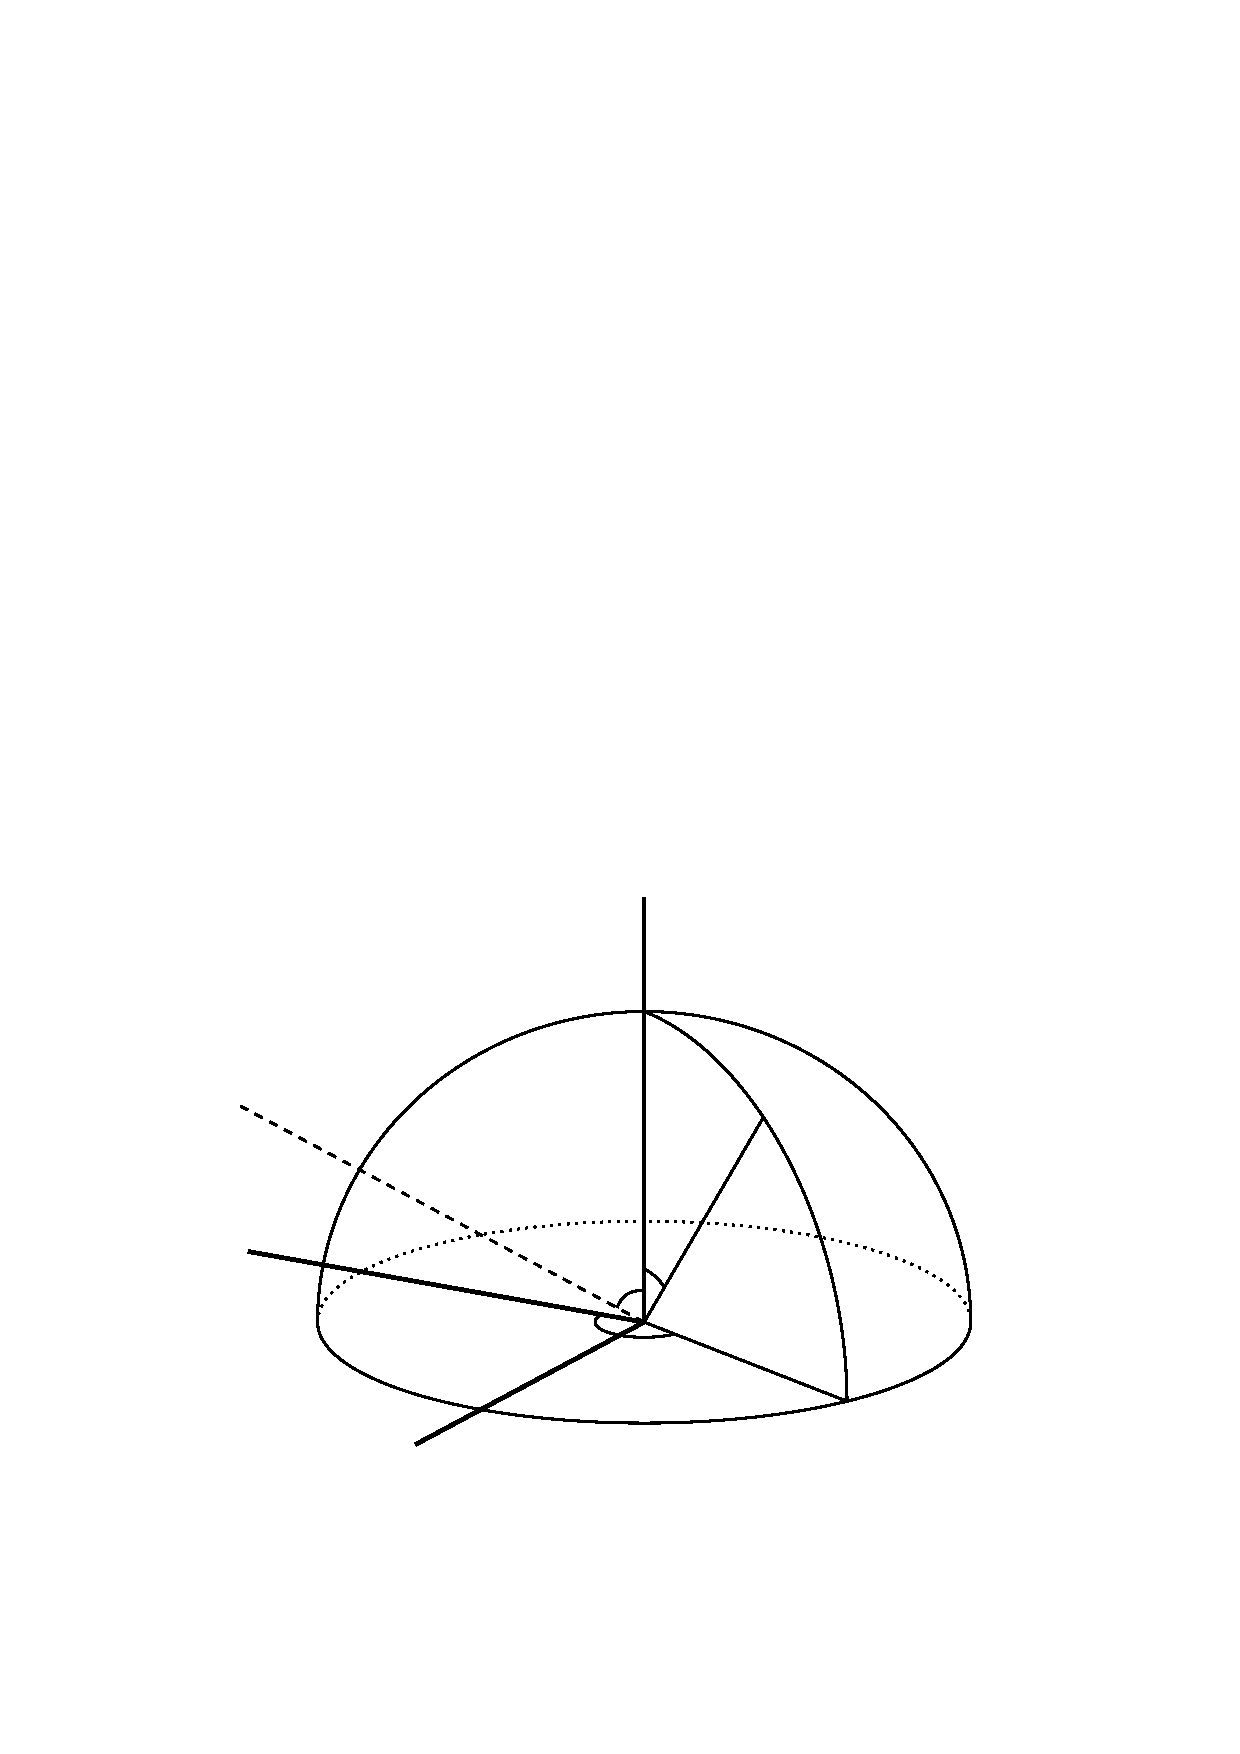
\includegraphics[width=9cm]{figs/fig1.pdf}
\caption{\label{fig:geom}
  Geometry of the system. Here we show the underlying spherical coordinate system with $\phi$ and $\theta$ coordinates along with the Cartesian $(x,y,z)$ coordinate frame.
In addition, the observers $\hat{x}-\hat{y}$ image plane is shown as viewed from an inclination angle $i$.
Star is also taken to rotate rapidly around the $y$ axis which leads to an oblate (squeezed) shape for the emitting surface, and, hence, the radial vector $\vec{r}$ and the surface normal $\vec{n}$ also start to differ from each other.
}
\end{figure}

Due to the rotation and finite pressure supporting the NS, it is not a perfect sphere when it is rotating.  
It, however, retains axisymmetry, and can be approximated with an oblate spheroid.  
Similarly to the second order space-time quantities, \citet{aGM14} derived an approximate shape of a rotating neutron star by expressing the radius as a function of colatitude $\theta$, as 
\begin{align}\begin{split}\label{eq:radf}
    R(\theta) &= \Req \left( 1 - \frac{\Req - R_{\mathrm{p}}}{\Req} \cos^2\theta \right) \\
              &= \Req (1-\Ob^2 (0.788 - 1.03x) \cos^2 \theta,
\end{split}\end{align}
where $R_{\mathrm{p}}$ is the radius on the rotational axis and $R(\pi/2) = \Req$.
Elemental surface area for a spheroid is given as (using the areal radial coordinates)
\be
dS(\theta) = R^2(\theta) \sin\theta \sqrt{1 + f(\theta)^2}d\theta d\phi,
\ee
where
\be
f(\theta) = \frac{1}{\bar{R}(\theta)} \frac{d \bar{R}(\theta)}{d \theta} 
= \Bb e^{-\zetab-\nub} \frac{1}{R(\theta)} \frac{dR(\theta)}{d\theta}, 
\ee
and $\Bb e^{-\zetab-\nub} \approx \left(1-\frac{2 G M}{c^2 r}\right)^{-1/2} + \mathcal{O}(\Ob^2)$.
The angle $\gamma$, defined as the angle between the radial unit vector $\vec{r}$ and the surface normal $\vec{n}$, is given by
\be
\cos\gamma = \left(1 + f(\theta)^2\right)^{-1/2}.
\ee
Then the normal to the surface can be defined using the radial vector $\vec{r}$ and the tangential vector $\vec{\theta}$ as
\be\label{eq:surf_norm}
\vec{n} = \cos\gamma \vec{r} + \sin\gamma \vec{\theta}.
\ee
See Fig.~\ref{fig:geom} for a clarification of the angles.



\subsection{Geodesic motion through Hamilton-Jacobi equation}\label{sect:hamjac}
Geodesic motion in a space-time characterized by a metric $g_{ij}$ is governed by Hamilton-Jacobi equation
\be\label{eq:hamjac}
2\frac{\pd S}{\pd \tau} = g^{ij} \frac{\pd S}{\pd x^i}\frac{\pd S}{\pd x^j},
\ee
where $g^{ij}$ is the inverse metric and $S$ denotes the Hamilton's principal function.
For the two Killing vectors $t^{\alpha} = (1,0,0,0)$ (asymptotic time symmetry) and $\phi^{\alpha} = (0,0,0,1)$ (rotational axisymmetry) in the rotating space-time, the Frobenius theorem implies the existence of a family of 2-surfaces orthogonal to these vectors \citep[see e.g.,][p.12]{rcs}.  
This means that there are surfaces of constant $t$ and $\phi$ in our spacetime, yielding two constants of motion, namely energy $E$ and the $z$-component of the angular momentum, $L_z$.  
We then seek a solution of equation~\eqref{eq:hamjac} in the form
\be
S = \frac{1}{2}\delta_1 \tau - Et + L_z\phi + S_{\rb}(\rb) + S_{\theta}(\theta),
\ee
where $\delta_1$ is related to the rest-mass of the particle we study.
With the metric function \eqref{eq:BWmetric} this becomes
\begin{align}\begin{split} 
    \delta_1 \rb^2 \Bb^2 e^{-2\nub} =~& \rb^2 \Bb^2 e^{-2\zetab} \pd_{\rb}S_{\rb}S^2 - e^{-4\nub} \Bb^2 \rb^2 (E - L_z \wb)^2 \\
                                & + \Bb^2 e^{-2\zetab} \pd_{\theta}S_{\theta}^2 + \frac{L_z^2}{\sin^2\theta}.
\end{split}\end{align}
After re-organizing terms and introducing a simplifying notation $e^{\zetab}/\Bb \equiv e^{\mub}$ we get
\begin{align}\begin{split}\label{eq:S}
& e^{-2\mub}\pd_{\theta}S_{\theta}^2 + \frac{L_z^2}{\sin^2\theta} = \\ 
& \Bb^2 e^{-2\nub}\rb^2 ( e^{2(\nub-\zetab)} \pd_{\rb}S_{\rb}^2 -\delta_{1} - e^{-2\nub}(E - L_z \wb)^2 ), 
\end{split}\end{align}
which is in a separated form, but only if $\nub = \nub(\rb)$, $\Bb = \Bb(\rb)$, $\zetab = \zetab(\rb)$ and $\mu = \mu(\theta)$.

To first order in rotation, i.e. $\mathcal{O}(\Ob)$, this condition is satisfied exactly because $e^{\mub} = 1 + \mathcal{O}(\Ob^2)$, in addition to $\nub = \nub_0(\rb) + \mathcal{O}(\Ob^2)$ and $\Bb = \Bb_0(\rb) + \mathcal{O}(\Ob^2)$ (see Table \ref{tab:coeffs}).  
In the second order of the expansion, $\theta$ dependent mass and pressure quadrupole moments are present, and separability is lost.
For geodesics, however, these higher order deviations only contribute very close to the actual NS surface, and neglecting them enables us to obtain accurate approximations of the photon path.

If we now assume separability, we can introduce a separation variable $\Ca$ known as Carter's constant (third constant of motion) in order to solve the differential equation \eqref{eq:S}.  
By noting that the conjugate momenta correspond to the first derivatives of $S$ with respect to the generalized coordinates, we can write the components of four-momentum, \fvec{p}, as 
\begin{align}
  p_t        &= -E \label{eq:p_t}\\
  p_{\rb}    &= \pm e^{\zetab - 2\nub} \left( \delta_1 e^{2\nub} + (E - L_z \wb)^2 - \frac{\Ca}{\Bb^2 e^{-4\nub} \rb^2} \right)^{1/2}\label{eq:p_r}\\
  p_{\theta} &= \pm e^{\mub} \left( \Ca - \frac{L_z^2}{\sin^2\theta} \right)^{1/2}\label{eq:p_the}\\
  p_{\phi}   &= L_z\label{eq:p_p}.
\end{align}
Similarly, the components of a local tetrad frame are
\begin{align}
  p^{(t)} &= -p_{(t)} = -e_{(t)}^{\hat{\mu}} p_{\hat{\mu}} = -e^{-\nub}p_t \label{eq:tetp_t}\\
  p^{(\rb)} &= p_{(\rb)} = e_{(\rb)}^{\hat{\mu}} p_{\hat{\mu}} = e^{-\zetab + \nub} p_{\rb} \label{eq:tetp_r}\\
  p^{(\theta)} &= p_{(\theta)} = e_{(\theta)}^{\hat{\mu}} p_{\hat{\mu}} = \frac{1}{\rb} e^{-\zetab+\nub} p_{\theta} \label{eq:tetp_theta}\\
  %p^{(\phi)} &= p_{(\phi)} = e_{(\phi)}^{\hat{\mu}} p_{\hat{\mu}} = -e^{-\nub} \wb p_t + \frac{1}{r \sin\theta} p_{\phi} \label{eq:tetp_phi},
  p^{(\phi)} &= p_{(\phi)} = e_{(\phi)}^{\hat{\mu}} p_{\hat{\mu}} = \frac{1}{e^{-\nub} \Bb \rb \sin\theta} p_{\phi} \label{eq:tetp_phi},
\end{align}
where $e^{\hat{\mu}}_{(a)}$ with index $a = t, \rb, \theta$ and $\phi$ are the tetrads of metric \eqref{eq:BWmetric}.
Since we only consider null geodesics (i.e. photons), we now set $\delta_1 = 0$.

\subsection{Ray tracing photons}\label{sect:raytracing}
Radiation is emitted from the surface of a star at an emission point $(r_e,\theta_e,\phi_e)$.  
The radiation travels along a geodesic with a specific intensity $I_{E}$ as measured by an observer co-moving with the emission point.  
It is observed at an image plane situated at a radial distance $r$, with $r\rightarrow\infty$.  
We then wish to calculate the projected image of the star at this image plane.

First we set up the coordinate system so that the plane of observation is towards $\phi = 0$ and $\theta = i$, where $i$ is the angle of inclination (see Fig.~\ref{fig:geom}).  
The geodesic will be emitted with a four-momentum $\fvec{p}_e$, and if it is eventually observed at the image plane at infinity, it will have a final four-momentum of $(E,\hat{p}_r,0,0)$, purely in the radial direction.  
Likewise, the components of the position must satisfy
\begin{align}
\theta &\rightarrow i \\
\phi   &\rightarrow 0,
\end{align}
as $r\rightarrow\infty$.
The change in the time and angular components along the geodesic can be written as
\begin{align}
dt      &= \frac{p^t}{p^{\rb}}\ud \rb \label{eq:deltatime} \\
d\theta &= \frac{p^\theta}{p^{\rb}}\ud \rb \label{eq:deltatheta} \\
d\phi   &= \frac{p^\phi}{p^{\rb}}\ud \rb \label{eq:deltaphi},
%d\theta &= \int_{r_e}^\infty \frac{p^\theta}{p^r}\ud r \label{eq:deltatheta} \\
%d\phi   &= \int_{r_e}^\infty \frac{p^\phi}{p^r}\ud r \label{eq:deltaphi},
\end{align}
yielding a total change of angles $\Delta\theta$ and $\Delta\phi$ when integrating from $r_e$ to $\infty$.
The condition for being observed is then
\begin{align}
\theta_e + \Delta\theta &= i \label{eq:thetacond}\\
\phi_e + \Delta\phi     &= 0 \label{eq:phicond}.
\end{align}

The projected image of the star on the image plane can then be described by two celestial coordinates:
abscissa $\hat{x}$ and ordinate $\hat{y}$.
Making use of the tetrad components \eqref{eq:tetp_t}--\eqref{eq:tetp_phi}, we obtain \citep[][p.347]{cha}
\be\label{eq:xhat}
\hat{x} = \left( \frac{rp^{(\phi)}}{p^{(t)}} \right)_{r \rightarrow \infty} = \frac{1}{\sin i} \frac{L_z}{E}
\ee
and
\be\label{eq:yhat}
\hat{y} = \left( \frac{rp^{(\theta)}}{p^{(t)}} \right)_{r \rightarrow \infty} = \frac{\sqrt{\Ca - \frac{L_z^2}{\sin^2 i}}}{E}.
\ee
Here it is useful to transform into a polar coordinate system on the image plane, as the equations \eqref{eq:xhat} and \eqref{eq:yhat} strongly suggest a more intuitive form if this is done. 
In this system we use as coordinates the radial distance from the center point, or the impact parameter $b$, and the polar rotation angle $\chi$.  
We take $\chi$ to increase clockwise from the projected spin axis of the neutron star, with $\chi=0$ corresponding to the projected direction from the south to the north pole of the neutron star.  
We then express the impact parameter $b$ and the angle $\chi$ via $L_z$ and $\Ca$ as%
\footnote{
    Here, the nature of Carter's constant as a generalized squared
    angular momentum is apparent.
}
\be
b = \frac{\sqrt{\Ca}}{E}
\ee
and
\be
\sin \chi = \frac{1}{\sin i} \frac{L_z}{\sqrt{\Ca}}.
\ee
The constants of motion, combined with the geodesic null condition $p^\mu p_\mu = 0$, allow us to solve $p^\theta$ and $p^\phi$ in terms of $\rb$.
As the final step we can substitute the four-momentum components and image-plane coordinates into \eqref{eq:deltatime}--\eqref{eq:deltaphi} and solve the system of three first-order differential equations (in terms of $t$, $\theta$ and $\phi$) with $\rb$ as a variable.


\subsection{Redshift and emission angle}\label{sect:redshift_angle}
It is most convenient to define all radiative processes in the co-rotating frame of the star.
We denote variables defined in a frame that is momentarily comoving with the stellar surface with a prime.  
On the other hand, our observer is stationary and moving along the timelike Killing vector.  
Hence, we need to transform between stationary and rotating frames by using the 4-velocity of the star's fluid.  
To make a connection to the theory of special relativity it is handy to define two frames: 
a co-rotating rest frame of the fluid $K'$ and a non-rotating static frame $K$.
Laws of physics for the radiative transfer take the usual form in the $K'$.
Observer, on the other hand, is located in the non-rotating frame $K$ from where the fluid is seen to move relativistically.
In addition, we need to take into account that a particle released from infinity with zero angular momentum will acquire nonzero angular velocity in direction of the star's rotation due to dragging of inertial frames.
Four-velocity of a stationary observer is then $o^{\alpha} = o^t(t^{\alpha})$, where the normalization factor $o^t = e^{-\nub}(1-\vw^2)^{-1/2}$ is obtained from $o_{\alpha}o^{\alpha} = -1$, and the velocity of the frame is 
\be
\vw = \wb \Bb e^{-2\nub} \rb \sin\theta,
\ee
indicating that the angular velocity as measured by an inertial observer at infinity is $o^{\phi} / o^{t} = d\phi/dt = \wb$.

A circular flow can be defined using the timelike and rotational Killing vectors as $s^{\alpha} = s^t (t^{\alpha} + \Omega \phi^{\alpha})$, where the normalization factor is defined as $s^t = e^{-\nub} (1 - \vz^2)^{-1/2}$ determined by $s_{\alpha}s^{\alpha} = -1$.
Here the velocity 
\be
\vz = (\Omega - \wb) \Bb e^{-2\nub} \rb \sin\theta,
\ee
can be identified as the 3-velocity measured in the frame of a zero angular momentum observer, an observer rotating along the frame with a velocity of $\vw$.

The total redshift as measured by an observed at infinity is then given by an inner-product between a photon $u^{\alpha}$ and a 4-velocity of the star's fluid $s^{\alpha}$.
With these definitions the redshift is
\be\label{eq:redshift}
1 + z = -s_{\alpha} u^{\alpha} = e^{-\nub} ~\delta^{-1},
\ee
consisting of the gravitational part $e^{\nub}$ and of the second Doppler-like term
\be
\delta = \frac{\sqrt{1-\vz^2}}{1 - \Omega L_Z}.
\ee

To compute the emission angle we again have to take the rotating frame into account.  
This can be done by introducing a projection operator $\bar{h}_{ab} = g_{ab} + s_a s_b$, which projects 4-vectors from the non-rotating frame to the rotating frame where the radiative processes are defined.  
As a definition, we can take the emission angle to be the angle between photon and a spacelike surface normal vector\footnote{
Line element in spherical coordinates is $d\vec{s} = dr \vec{\hat{r}} + r d\theta \vec{\hat{\theta}} + r \sin\theta d\phi \vec{\hat{\phi}}$ and by combining this with equation \eqref{eq:surf_norm} we obtain the presented surface normal.
}
$n_{\alpha} = (0, \cos\gamma/N_n, \rb \sin\gamma/N_n, 0)$, with normalization $N_n = e^{\zetab - \nub}$ fulfilling $n_{\alpha}n^{\alpha} = -1$.  
When projected to the rotating-frame we can then obtain the angle from the generalized dot-product definition between two vectors as
\be\label{eq:gen_angle}
\cos\alpha' = \frac{\bar{h}_{ab}n^a u^b}{(\bar{h}_{ab} n^a n^a)^{1/2} (\bar{h}_{ab} u^a u^b)^{1/2}}.
\ee
Using the metric defined by \eqref{eq:BWmetric} and a photon with components \eqref{eq:p_t}$-$\eqref{eq:p_p}, we obtain
\be\label{eq:cosap}
\cos\alpha' = \delta e^{2\nub-\zetab} \left[ p_{\rb} \cos\gamma + \frac{p_{\theta}}{\rb}\sin\gamma \right].
\ee
For the non-rotating observer we similarly obtain 
\be\label{eq:cosa}
\cos\alpha = \cos\alpha' \delta^{-1}.
\ee
Here it suffices to notice that we are only interested in the emission angle value at the surface of the star i.e. $\rb = \bar{R}(\theta)$.
The result here is similar to the emission angle obtained with a special-relativistic approach, using flat-space trigonometry and Lorentz-boosting to the rotating frame \citep[see e.g.,][]{PB06}.


\subsection{Emission}\label{sect:emission}
Observed (i.e., received) flux at photon energy $E$ from a small area on an image plane is
\be
dF_E = I_E d\Omega_o,
\ee
where $I_E$ is the specific intensity of the radiation at infinity and $d\Omega_o$ is the solid angle subtended by the element as measured by the observer. 
The total flux is then the integral of these elements over the image plane.
As a final step this observed flux has to be connected to the actual emerging radiation.

From equation~\eqref{eq:redshift}, the relation between the emergent energy $E'$ to the observed energy $E$ is $E/E' = (1 + z)^{-1}$.
The connection between the monochromatic observed and local intensity is then (see e.g. \citealt{MTW73}, p.588; \citealt{RL79}, p.145)
\be
I_E = \left( \frac{E}{E'} \right)^3 ~I'_{E'}(\alpha'),
\ee
where $I'_{E'}(\alpha')$ is the intensity computed in the frame comoving with the emitting area.
The radiation here is emitted in the direction of the emission angle $\alpha'$ defined in the local rotating frame.
Integrating over the energies, we get the bolometric intensity
\be
I = \left(\frac{E}{E'} \right)^4 ~I'(\alpha').
\ee
The total (monochromatic) flux as a function of observer's time $F_E(t)$ can then be obtained by integrating over the whole image
\be\label{eq:fluxint}
F_E(t) = \int I_{E}(t) ~d\Omega_o = \int\int \frac{I'_{E'}(t_*, \alpha')}{(1+z)^3}  ~\frac{bdb \, d\chi}{D^2}
\ee
where $t_* = t - \Delta t$ is the time when the photon was originally emitted. 
This can be computed when we know the total travel time $\Delta t$ against some reference photon, for example the one with the shortest path to the observer.

All of these quantities on the star's spherical coordinate system $(\theta, \phi)$ are then mapped to the observers polar image coordinates $(b, \chi)$ via ray tracing.
Note that the original longitudinal coordinate of the emission is easily obtained from $\phi_e = \phi - t_* \Omega$, because both $t_*$ and $\Omega$ are defined for a distant observer and change in the azimuthal coordinate is Lorentz invariant.
%This mapping $(b, \chi) \rightarrow (\theta, \phi)$ allows us to then evaluate the physical quantities
%\begin{align}
%1+z                  &\rightarrow 1+z(\theta, \phi) \rightarrow 1+z(b, \chi), \\
%\cos\alpha'          &\rightarrow \cos\alpha'(\theta, \phi) \rightarrow \cos\alpha'(b, \chi), \\
%\Delta t             &\rightarrow \Delta t(\theta, \phi) \rightarrow \Delta t(b, \chi), \\
%I'_{E'}(t_*, \alpha') &\rightarrow I'_{E'}(t_*, \cos\alpha'; \theta, \phi) \rightarrow I'_{E'}(t_*, \cos\alpha'; b, \chi)
%\end{align}
%in the observers plane for the flux calculations.

\subsection{Co-rotating coordinate frame}\label{sect:coords}
Next we define some quantities for a co-rotating observer.
Moving from the observers non-rotating frame $K$ to the fluids rest frame $K'$ is easily done using the previously defined projection operator $\bar{h}_{ab}$. 
Our metric tensor for the rotating observer is 
\be
\bar{h}_{ab} dx^a dx^b = e^{2(\zetab - \nub)} (d\rb^2 + \rb^2 d\theta) + \frac{\Bb^2 e^{-2\nub} \rb^2 \sin^2\theta}{1-v_Z^2} d{\phi'}^{2},
\ee
where we have defined a new angular coordinate $\phi' = \phi - \Omega t$ that is used by the rotating observer.%
\footnote{We thank S. Morsink for pointing this out.}
It is important to notice here that because of the rotation the azimuthal angle $\phi$ and the time $t$ are now coupled for the co-moving observer.
The normalized longitudinal coordinate ensures that both, rotating and stationary observer, agree that a circle drawn around the star has $2\pi$ radians.
This new longitudinal coordinate is also seen to be Lorentz contracted by a factor of $\gamma_\mathrm{L} = (1-\vz^2)^{-1/2}$.

Next we move to a normal (areal) \sch coordinate system so that the emission regions with similar coordinate extents at different latitudes have the same area.
By using the equations \eqref{eq:rb2r} and \eqref{eq:drb2dr} we obtain a longitudinally Lorentz-boosted metric tensor 
\be \label{eq:gammaSch} 
h_{ab} dx^a dx^b = e^{-2\nub}dr^2 + \frac{e^{2\zetab}}{\Bb^2} r^2 d\theta + \lgamma^2 r^2 \sin^2\theta d{\phi'}^2.
\ee 
%where $\gamma_\text{L}$ is the Lorentz boost factor.
The result agrees with (areal) \sch coordinate system up to first order in rotation due to the fact that $e^{\zetab}/\Bb \approx 1 + \mathcal{O}(\Ob^2)$.  
Additionally we can drop the gravitational redshift term $e^{-2\nub}$ of the radial coordinate because we do not consider any finite height for the system later on.
Next we can define a radial vector in (3D) Cartesian coordinate system as 
\be
\vec{r} = (x_r, y_r, z_r) = r (\cos\phi' \sin\theta, \sin\phi' \sin\theta, \cos\theta).
\ee
%where normalization factor $\hat{R} = \sqrt{x_r^2 + y_r^2 + z_r^2}$.
By using the Jacobian $\partial(x_r, y_r, z_r)/\partial (r, \theta, \phi')$ the spherical coordinate system \eqref{eq:gammaSch} can be transformed into a Cartesian coordinate basis, and by setting $\phi'=0$ we define our frame with $y$-axis along the direction of the motion, $x$-axis along the meridian towards the equator, and $z$ axis along the radial direction.
Hence, the co-rotating observer has a Cartesian metric%
\footnote{ It is also possible to generalize the Cartesian basis for oblate surfaces by considering a projection operator $\hat{h}_{ab} = g_{ab} + s_a s_b - n_a n_b$ with an additional projection against $n_a$, which is the normal to the (oblate) surface.
}
\begin{align}\begin{split}
%&\hat{g}_{ij} dx^i dx^j &= \frac{\partial(r, \theta, \phi_*)}{\partial{(x, y, z)} h_{ab} dx^a dx^b  \\
    & \hat{g}_{ij} d\hat{x}^i d\hat{x}^j = \frac{\partial x^a}{\partial \hat{x}^i} \frac{\partial x^b}{\partial \hat{x}^j} h_{ab} dx^a dx^b  \\
&= \gamma_L^2 dy^2 + \frac{1}{2} \Biggl[ \Bigl(1+ \frac{e^{2\zetab}}{\Bb^2}\Bigr)(dx^2 + dz^2) \\
&+ \Bigl(\frac{e^{2\zetab}}{\Bb^2} - 1\Bigr)(dx-dz)(dx + dz) \cos(2\theta) - 2dx dz \sin(2\theta) \Biggr] \\
& = dx^2 + \gamma_L^2 dy^2 + dz^2 + \mathcal{O}(\Ob^2)
\end{split}\end{align}
From the Cartesian form of the co-rotating metric it is also easy to obtain the great circle distance (on a unit sphere) as measured by the co-rotating observer by using the generalized inner-product \eqref{eq:gen_angle} as
\be\label{eq:rel_cos}
\cos\rho' = \frac{\cos\theta \cos\theta_\mathrm{S} + \cos\phi \sin\theta \sin\theta_{\mathrm{S}}}{\sqrt{ \cos^2\theta + \sin^2\theta (\cos\phi^2 + \lgamma^2 \sin\phi^2)}} + \mathcal{O}(\Ob^2),
\ee
This is the angle between points $(\theta, \phi)$ and $(\theta_{\mathrm{S}}, 0)$, and can be used to define the \textit{angular} size of spots as measured by the co-rotating observer in $K'$.
Note that the circumference of the star as measured by this co-rotating observer is now $>2\pi R$ because the azimuthal direction is Lorentz stretched.

%%%%%%%%%%%%%%%%%%%%%%%%%%%%%%%%%%%%%%%%%%%%%%%%%%
Quantities here are also relevant for the so-called Schwarzschild+Doppler (S+D) approximation \cite[see e.g.,][]{PB06}.
In the S+D approximation the observers polar coordinate plane $(b,\chi)$ is connected to the co-rotating spherical coordinates $(\phi', \theta')$ of the star.
In this method, the calculations are done in a special relativistic framework assuming infinitesimally small spots.
We will now show how to expand this approximation to a full general relativistic exact form valid also for finite sized spots (see also \citealt{CML07}, for an alternative derivation).
In (areal) \sch metric the impact parameter $b$ can be obtained as a function of the emission angle $\alpha$ \eqref{eq:cosa} as
\be
%b = e^{-2\nu} R \sin\alpha.
b = \frac{1}{\sqrt{1-u}} R \sin\alpha.
\ee
by setting $\cos\gamma \rightarrow 1$, $\sin\gamma \rightarrow 0$ (spherical star), and $\omega \rightarrow 0$ along with $e^{-2\nu} \rightarrow (1-u)^{-1/2}$ (\sch metric, i.e., $\mathcal{O}(\Ob^1)$).
Note that here we use the emission angle as measured by the non-rotating observer in frame $K$.
In this case, the solid angle is then simplified to 
\be
d\Omega_o = bdb \, d\chi = \frac{1}{1-u} \frac{d \cos\alpha}{d \cos\psi} R^2 \cos\alpha ~ \frac{d\chi d\cos\psi}{D^2},
\ee
where $\psi$ is the lensing angle.
Using the symmetry of the \sch metric we can then directly connect the $\psi$ and $\theta$ along with $\chi$ and $\phi$ to obtain
\be
d\Omega_o = \frac{1}{1-u} \frac{d \cos\alpha}{d \cos\psi} ~\cos\alpha ~ \frac{dS}{D^2},
\ee
where $dS = R^2 d\cos\theta d\phi$ is the area element for the non-rotating static observer in $K$.
Using $d\Omega_o$ to compute the flux we would then get the observed (received) flux valid for the observer in frame $K$.

Integration over some finite sized features, on the other hand, is done on top of the surface of the star in the co-rotating frame $K'$.
This results in a mixing of the different frames because we would like the integration to happen simultaneously for the observer in $K$, i.e., we need a connection between $t$, $\phi$ and $\phi'$.
From the projection operator we can work out the total differential area element as
\begin{align}\begin{split}\label{eq:dSp}
dS' &= \sqrt{\det h_{ab}} d\theta d\phi d t\\
%&= \frac{e^{\zetab}}{B} \lgamma r^2 \sin\theta d\theta d\phi' = \lgamma d\cos\theta d\phi' + \mathcal{O}(\Ob^2). \\
&= \frac{e^{\zetab}}{B} \lgamma R^2 \sin\theta d\theta d\phi' = \lgamma R^2 d\cos\theta d\phi' + \mathcal{O}(\Ob^2).
%&= \lgamma dS'' + \mathcal{O}(\Ob^2).
\end{split}\end{align}
%\red{TODO: In which coordinates is $dS''$ defined now? We had two frames (= coordinate systems), $K$ and $K'$. In which coordinate frame is $dS''$ defined?}
Hence, a change of $t$ and $\phi$  will result in a stretching of the area element by a factor of $\lgamma$.
This result is obtained purely from differential geometry.

Next we will work only in the \sch case and consider only terms up to $\mathcal{O}(\Ob^2)$.
To transform from the non-rotating $K$ frame to the co-rotating frame $K'$ we can use the Lorentz invariance of the photon beam cross-section given as \citep{Terrell60, LB85}
\be
\cos\alpha ~dS = \cos\alpha' ~dS'.
\ee
%This follows from the fact that the photon beam cross-section is Lorentz invariant, i.e., $\cos\alpha ~dS = \cos\alpha' ~dS'_o$.
Connection between the emission angles $\cos\alpha'$ and $\cos\alpha$ is also known from equations \eqref{eq:cosap} and \eqref{eq:cosa} and is seen to be a simple Doppler boost factor $\delta$.
From here we then obtain
\be
dS = \lgamma \delta R^2 \sin\theta d\theta d\phi',
\ee
as given by the co-rotating frame coordinates.
%when taking into account also the transformation of frames $K$ and $K'$ using the differential area from \eqref{eq:dSp}.
%A possible misconception here might arise from the fact that the power emitted is Lorentz invariant but the power received is not \citep[see e.g.][]{Ghi99}!
Finally, the total observed angular size is then seen to be 
\be
d\Omega_o = \frac{\lgamma \delta}{1-u} \frac{d \cos\alpha}{d \cos\psi} ~\cos\alpha ~ \frac{R^2 \sin\theta d\theta d\phi'}{D^2}.
\ee
%as given by the co-rotating frame coordinates $dS'' = R^2 d\cos\theta d\phi'$.
%\red{TODO: This should be clarified. What does ``simultaneous measurements of local static observers'' mean? Same thing for ``Simultaneous measurements made by different static observers are not simultaneous for moving observers due to the coupling between time and space.'' Simultaneity and GR is very elusive and mostly poorly defined. The referee wil give us an ass-kicking if we're not super exact and careful here.}
It differs by a factor of $\lgamma$ from the S+D approximation that is valid for an infinitesimally small spots.
In special relativity we could say that the surface element $dS'$ must be defined based on simultaneous measurements of local \textit{static} observers --- not using simultaneous measurements of comoving observers --- when dealing with finite sized spots on the surface.
Simultaneous measurements made by different static observers are not simultaneous for moving observers due to the coupling between time and space.
Hence, ray tracing photons from the observer to the star and using the frame of the static observer our time coordinate is automatically correct and the difference is seen in the size of the spots (see eq. \ref{eq:rel_cos}).
Working in the co-rotating frame $K'$ the lengths (i.e., spot size and shape) are taken to be correct and it is a question of how to connect the time intervals to the observers time measurements.
Here the error in time might then be interpreted as not taking into account the different photon arrival times to the detector.


\subsection{Angular distribution of radiation}\label{sect:angular_distr}
\subsubsection{Isotropic radiation}

For pulse profile calculations the simplest angular distribution of radiation is the isotropic radiation.
Here we consider blackbody emission described by the specific intensity
\begin{equation}
  B_{\mathrm{E}}(T) = 5.04 \times 10^{22} \frac{E^3}{\mathrm{exp}(E/T) -1}~\mathrm{erg}\,\mathrm{s}^{-1}\,\mathrm{cm}^{-2}\,\mathrm{keV}^{-1}\,\mathrm{sr}^{-1},
\end{equation}
where $T$ and $E$ are given in keV.
The radiation is isotropic and there is no dependence on the angle $\alpha'=\cos^{-1}\mu'$, measured relative to the surface normal by the co-rotating observer.

\subsubsection{Electron scattering dominated atmosphere}

The second angular distribution we consider is the so-called `Hopf profile', which is no longer isotropic.
The spectral distribution is still given by the Planck function, but the angular distribution is assumed to be produced in a coherent electron scattering dominated plane-parallel semi-infinite (optical depth $\tau \rightarrow \infty$) atmosphere.
The result is
\begin{equation}
  I_{\mathrm{E}}(\mu) = B_{\mathrm{E}}(T) \frac{H(\mu)}{2\alpha_1},
\end{equation}
where
\begin{equation}
  \alpha_n = \int_0^1 H(\mu) \mu^n d\mu
\end{equation}
are the moments of the function $H(\mu)$, which is a solution of the Ambartsumian-Chandrasekhar integral equation \citep[see e.g.][]{Cha60,Sob63}
\begin{equation}\label{eq:hmu}
  H(\mu) = 1 + \mu H(\mu) \int_0^1 \frac{\Psi(\eta)}{\mu + \eta} H(\eta) d\eta.
\end{equation}
Here $\Psi(\mu)$ is the characteristic function, which depends on the scattering law considered.
For Rayleigh (Thomson) scattering it is
\begin{equation}
  \Psi(\mu) = \frac{3}{16}(3-\mu^2).
\end{equation}
Given $\Psi$, the integral equation \eqref{eq:hmu} can then be iteratively solved, for example, by computing
\begin{equation}\begin{split}
    H_{n+1}(\mu) =  \frac{1}{2} H_n(\mu) + \frac{1}{2}\Biggl(& \sqrt{1-2\int_0^1 \Psi(\eta)d\eta} \\
                    &+ \int_0^1 \frac{\eta \Psi(\eta)}{\mu + \eta} H_n(\eta) d\eta \Biggr)^{-1},
\end{split}\end{equation}
with a starting guess of
\begin{equation}\label{eq:apprx_hopf}
  H_0(\mu) = 1 + 2.3\mu - 0.3\mu^2.
\end{equation}
We also note that even the simple polynomial expansion \eqref{eq:apprx_hopf} already has an accuracy better than $<2\%$, and as such it can be used in approximate solutions with a corresponding first moment of $\alpha_1 = 1.19167$.


\subsection{Method of solution}\label{sect:num_methods}


\begin{figure}
\centering
\includegraphics[width=8cm]{figs/fig6a.pdf}
%\includegraphics[width=7cm]{figs/fig6b.pdf}
\caption{\label{fig:grid}
Example of a non-equidistant polar grid used in our ray tracing with $N_r = 20$ and $N_{\chi} = 30$ points.
Red dashed line corresponds to the outline of the actual oblate star that is covered with a chess board pattern.
}
\end{figure}

In practice we trace the photons from the image plate at infinity all
the way to the surface of the star by solving the first order
differential equations \eqref{eq:deltatime}--\eqref{eq:deltaphi}
backwards in time.  In addition, we make a simple variable substitution $\tilde{x} = 1/r$
 that will help us by stretching the step when
far from the star and shortening it when coming close to the star
surface.  Here an adaptive step size second order Heun's Runge-Kutta
integrator is used with forward Euler's method as
the predictor and trapezoidal method as the corrector.  
All photons that travel
more than $0.95\tilde{x}$ away from the star after a U-turn are
terminated and considered to have missed the star.

Our image plate is defined using a polar coordinate system with a radial
coordinate $b$ (i.e., the impact parameter) and an angular coordinate $\chi$.
We also employ a non-equidistant grid in both coordinates to accommodate
the extra resolution needed around the edges of the star.  Radial
coordinate $b$ is defined using a Gauss-Laguerre abscissa (i.e.,
$e^{-b}$-weighted) and the angle coordinate is weighted with a simple
sinusoidal function so that the resolution is increased around the top
and bottom parts where $\chi = 0$ or $\pi$, which is near the location of the poles
(see Fig.~\ref{fig:grid}).  By ray tracing we then obtain
a mapping between the image plane and the surface of the star, defined
on a grid.
Arbitrary positions in the image plane are 
obtained by a linear interpolation in $(b, \chi)$ space.

For pulse profile calculations where only a small part of the star is
emitting we first search a crude location of the spot on the image plane
and then impose a fine subgrid around it in order to accurately
calculate the flux from this small patch.  The subgrid itself is defined
either in polar grid (by constraining minimum and maximum $\chi$ and
$b$) or in Cartesian image grid (by constraining minimum and maximum
$\hat{x}$ and $\hat{y}$) depending on the total area covered in the observers sky.  To
calculate the total flux $F(t)$ we then integrate this small subgrid by
using an adaptive multidimensional integration.  The algorithm is based
on a tensor product of nested Clenshaw-Curtis quadrature rules and is
implemented using the \textsc{Cubature} package.\footnote{
\url{http://ab-initio.mit.edu/wiki/index.php/Cubature}}





%%%%%%%%%%%%
\section{Applications \& Validation}\label{sect:appl}

Next we present some applications of the framework to some simple physical problems related to neutron stars to showcase the possibilities that one can utilize the code for.
The examples are also meant to act as a further validation, as we provide a comparison with existing literature results, when possible.
Most notably, we employ an extensive comparison against AMP pulse profiles computed with a code that propagates photons forward in time as presented in \citet{PB06} and in Sect.~\ref{sect:coords}.
As such, our code serves as a great cross-validation tool for these kind of special relativistic formulations because our framework is fully general relativistic and propagates photons backwards in time from the observer to the surface.



\subsection{Images of neutron stars}

\begin{figure*}
\centering
\includegraphics[clip, trim=0.0cm 0.5cm 0.0cm 2.0cm, width=8cm]{figs/fig10a.pdf}
\includegraphics[width=7cm]{figs/fig10b.pdf}
\caption{\label{fig:image}
  Formation of an image in curved spacetime.
  Left panel shows a 3D visualization of the photon trajectories in the curved spacetime starting from the star and ending to the observers image plane.
  Right panel shows the image that the observer sees using the Cartesian $\hat{x}$ and $\hat{y}$ coordinates.
  For illustrative purposes the neutron star surface is covered with a chess board pattern.
  }
\end{figure*}


As a first application of the code, we can determine the photon trajectories using the ray tracing algorithm and produce an image of the neutron star as seen by the observer.
This also shows how we can connect the Cartesian coordinates $\hat{x}$ and $\hat{y}$ of the observer to the coordinates $\phi_e$ and $\theta_e$ of the star.
Left panel in Fig.~\ref{fig:image} shows the trajectory of the photons in 3D, using a $\hat{z}$-coordinate in addition to the Cartesian image plane coordinates $\hat{x}$ and $\hat{y}$.
The star is chosen to have $R=12~\mathrm{km}$ and $M=1.5~\Msun$, whereas the observer is located at the equator with an inclination of $i = 90^{\circ}$.
Here the photons originate from the image plane located at $\hat{z} = 20$ and are then propagated backwards in time until they intersect with the surface of the star (center of the star located at $\hat{z} = 0$) , visualized with a spherical see-through wiregrid frame.
Right panel of the figure shows the projected image as seen by a distant observer.
Here the star is covered with a chess board pattern to show how the $\phi_e$ and $\theta_e$ coordinates on the neutron star surface are seen by the distant observer.


\subsection{Accuracy of the split Hamilton-Jacobi propagator}

\begin{figure*}
\centering
\includegraphics[width=16cm]{figs/popiha/fig_casual_15.pdf}
\includegraphics[width=16cm]{figs/popiha/fig_casual_45.pdf}
\includegraphics[width=16cm]{figs/popiha/fig_casual_75.pdf}
\includegraphics[width=16cm]{figs/popiha/fig_extreme_15.pdf}
\includegraphics[width=16cm]{figs/popiha/fig_extreme_45.pdf}
\includegraphics[width=16cm]{figs/popiha/fig_extreme_75.pdf}
%\includegraphics[width=18cm]{figs/popiha/casual_400pts_16m_12km_400hz_15inc.pdf}
%\includegraphics[width=18cm]{figs/popiha/casual_400pts_16m_12km_400hz_45inc.pdf}
%\includegraphics[width=18cm]{figs/popiha/casual_400pts_16m_12km_400hz_75inc.pdf}
%\includegraphics[width=18cm]{figs/popiha/extreme_400pts_14m_15km_600hz_15inc.pdf}
%\includegraphics[width=18cm]{figs/popiha/extreme_400pts_14m_15km_600hz_45inc.pdf}
%\includegraphics[width=18cm]{figs/popiha/extreme_400pts_14m_15km_600hz_75inc.pdf}
\caption{\label{fig:H_C1_C2}
    Errors in ray tracing two neutron stars with $R=12\,\mathrm{km}$, $M=1.6\Msun$, $\nu=400\,\mathrm{Hz}$ or $R=15\,\mathrm{km}$, $M=1.4\Msun$, $\nu=600\,\mathrm{Hz}$, and with observer inclinations $i=15^\circ$, $45^\circ$ and $75^\circ$, using the \textsc{arcmancer} code.
    The leftmost panels show the maximal variation in the Hamiltonian $H$ of the geodesic, while the center and rightmost panels show the maximal variation in the Jacobi constant, computed either with the left side ($C_1$) or the right side ($C_2$) of equation \eqref{eq:S}.
  }
\end{figure*}

Next, we study the feasibility of the split Hamilton-Jacobi propagator by comparing to results from a general-purpose geodesic solver \textsc{arcmancer} (Pihajoki et al. 2016, \emph{in prep.}).
The comparison solver directly solves the Lagrangian equations of motion of the geodesic in an arbitrary user-given metric. 
We compute the change in the Jacobi constant as computed with both sides of equation \eqref{eq:S}, and the change in the value of the Hamiltonian of the geodesic for two different neutron star configurations:
$R=12\,\mathrm{km}$, $M=1.6\Msun$, $\nu=400\,\mathrm{Hz}$, and $R=15\,\mathrm{km}$, $M=1.4\Msun$, $\nu=600\,\mathrm{Hz}$.
Observer inclinations considered are $i=15^\circ$, $45^\circ$ and $75^\circ$.
The results are shown in Figure~\ref{fig:H_C1_C2}. In general, we see that the assumption of separability, as measured by the variation in the Jacobi constant, is good to a level of $10^{-3}$--$10^{-2}$, except for geodesics that hit the center of the neutron star from the observer's point of view. However, the examples were deliberately chosen to be extreme, and the approximation of separability is much better for more slowly rotating neutron stars.
We further note that in cases of extreme rotation or when high precision is required, the geodesic propagation can easily be done using the \textsc{arcmancer}, instead of equations \eqref{eq:deltatime}--\eqref{eq:deltaphi}, while using the rest of the results in this paper for the actual radiation computations.

\subsection{Line profiles}

\begin{figure}
%\centering
\includegraphics[width=8cm]{figs/fig9a.pdf}
%\includegraphics[width=8cm]{figs/fig9b.pdf}
\caption{\label{fig:line_profiles}
  Observed line profiles from a star with $R=10~\mathrm{km}$ and $M=1.4~\Msun$ rotating with a frequency of $700~\mathrm{Hz}$.
  A normal spherical star with \sch spacetime is shown with a black line while an oblate ($R_{\mathrm{e}}=10~\mathrm{km}$) star in a same spacetime is shown with a blue line.
  Oblate star with a non-zero quadrupole moment is presented with a red solid line while the red dashed line shows the line profile of a star with an artificially enhanced quadrupole moment of $q \times 5$.
  }
\end{figure}


\begin{figure}
%\centering
\includegraphics[width=8cm]{figs/fig9c.pdf}
\caption{\label{fig:line_profiles_sweep}
  Observed line profiles from stars with $M = 1.4~\Msun$, $i = 20^{\circ}$, and a varying radius for a rotational frequency of $700~\mathrm{Hz}$.
  Star's oblate shape is computed according to \eqref{eq:radf} and the spacetime has non-zero quadrupole moments as given by \eqref{eq:quad}~ and \eqref{eq:beta}.
  }
\end{figure}

As a next step, we can study the energy dependent flux from the star by computing the observed energy distribution $E$ for a delta injection of energy $E'$ from the surface.
Because of the varying redshift along the surface of the star due to Doppler boosting, the observer then sees a range of energies \citep{OP03,BML06,CMB06}.
Examples of line profiles are shown in Fig.~\ref{fig:line_profiles} for different spacetimes and star configurations.
The flux is normalized so that the emitted bolometric flux is unity, i.e., the area encapsulated by the profile is one.
In each case, the star is taken to have $\nu = 700~\mathrm{Hz}$, $R = 10~\mathrm{km}$, and $M=1.4~\Msun$.
Observer inclination is $i=20^{\circ}$ and emission is taken to be proportional to $(E/E')^3$ with an isotropic beaming for simplicity.
We consider a \sch spacetime for spherical and oblate stars, with radius given by equation~\ref{eq:radf}, in addition to a full second-order spacetime with quadrupole moments and an oblate neutron star surface.

The obtained profiles can be compared to the ones in Fig.~2 of \citet{BPO13} where the \sch results are seen to match well with our calculations.
For the second-order metric we see a deviation due to the differing value of the quadrupole moments:
In the Hartle-Thorne metric \citep{HT68} the quadrupole moment is given by $q = -a^2 (1 + \eta)$, where $a$ is the dimensionless spin parameter (see eq. \eqref{eq:wbar} and our $j$) and $\eta$ is the strength of the deviation from a spherical potential ($\eta = 0$ reduces to Kerr-like spacetime).
\citet{BPO13} select $\eta=3.3$ that is a typical value given by the FPS EoS \citep{FPS} for a star with $M\approx1.4~\Msun$ \citep[see][]{LP99}.
For the angular momentum they adopt $a = 0.357$, again, as given by the FPS EoS at $\nu \approx 700~\mathrm{Hz}$.
With the aforementioned value, their quadrupole moment is then $q \approx -0.548$.

The quadrupole moment is larger for a stiffer EoS, because a stiffer EoS produces a larger star and the quadrupole moment scales with the square of the radius.
For us, this scaling is taken into account by the relations \eqref{eq:quad} and \eqref{eq:beta} that are obtained by fitting a large library of EoSs \citep[see][]{aGM14} to yield a consistent quadrupole moment at any given mass, radius (i.e., stiffness) and angular velocity.
This scaling also hides the difference between the non-rotating and rotating radii because it is formulated using the equatorial radius $R_{\mathrm{e}}$.
Alternatively, one could always consider the corresponding $R_0$ of a non-rotating configuration for which $R_0 \le R_{\mathrm{e}}$ for any given $\Ob$.
For a $M=1.4~\Msun$, $R_{\mathrm{e}}=10~\mathrm{km}$, and $\nu = 700~\mathrm{Hz}$ we obtain $j \approx 0.275$, $q \approx -0.268$, and $\beta \approx 0.010$ that then give $\qinv \approx -0.255$.
Additionally, a star like this with $\Ob \approx 0.323$ has an eccentricity $\epsilon \approx 0.341$ as given by the radius function \eqref{eq:radf}.
Line profile emerging from a such a star is shown with a red solid line in Fig.~\ref{fig:line_profiles} and is not seen to develop a narrow core because the quadrupole moment is not strong enough to dominate over the gravitational part $e^{\nub_0}$ in the $g_{tt}$ component of the metric.
By artificially enhancing the quadrupole moment to be $q \times 2$, roughly consistent with the value used in \citet{BPO13}, we do reproduce the narrow feature in the blue part of the line profile for a spherical star.
For an oblate star, we need $q \times (4-5)$ for the line profile to produce a narrow core as seen in the red dashed line in Fig.~\ref{fig:line_profiles}.
Here the large difference to the spherical configuration is explained by the increasing eccentricity of the star that acts as a countering force because it strengthens the gravitational part of the $g_{tt}$ component due to the star being more compressed, and hence more compact, around the poles.

On the other hand, by adopting $M = 1.4~\Msun$, $j = 0.357$ and $\nu = 700~\mathrm{Hz}$, our radius is fixed to be $R_{\mathrm{e}} \approx 11.8~\mathrm{km}$.
This results in an eccentricity of $\epsilon \approx 0.444$, $\beta \approx 0.013$, $q \approx -0.613$, and $\qinv \approx -0.595$, consistent with the values given by the FPS EoS as tabulated by \citet{LP99} for $q$ and by \citet{CST94} for the rest of the parameters.
Note also that $R_0 = 10.85~\mathrm{km}$ for $M=1.4~\Msun$ with a stiffness given by the FPS EoS \citep{CST94}.
No narrow core is seen to form in this case either as it is always the increasing gravitational part of the $g_{tt}$ near the compressed poles that counters the increasing quadrupole moment with increasing eccentricity.
In fact, no narrow core is ever seen to form when the oblateness and quadrupole moments are computed in a consistent way, as above.
To validate this, we computed line profiles for a range of $R_{\mathrm{e}}$ ranging from $10$ to $16$ km as shown in Fig.~\ref{fig:line_profiles_sweep} for $M=1.4~\Msun$.
No deviations from the overall rather smooth profile is seen even for the extreme case of $M = 1.1~\Msun$ where we expect to maximize the quadrupole moment of the configuration.



\subsection{AMPs pulse profiles}\label{sect:AMPs}

From here on, we move to time-dependent ray tracing problems by considering pulse profiles from AMPs.
Here a hot spot on top of the surface is emitting and the star is seen to rotate with a frequency of $\Omega$.


%\subsubsection{Schwarzchild $+$ Doppler}

First, a general comparison of the ray tracing algorithm with the S+D approximation \citep{PB06} was done (see also Sect.~\ref{sect:coords}).
For simplicity, only spherical stars were considered here.
Main parameters were: the stellar mass $M = 1.6~\Msun$, the stellar radius $R = 12~\mathrm{km}$, the observer inclination $i = 60^{\circ}$ and the colatitude of the spot $\theta_{\mathrm{s}} = 50^{\circ}$.  
The effective temperature of the radiation was set to $T_{\mathrm{eff}} = 2~\mathrm{keV}$.  
The distance to the source was assumed to be $D = 10~\mathrm{kpc}$.  
We defined a circular spot with an angular radius $\rho$ of either $1$ or $30$ degrees.
Here the spot is defined using an angle as measured by the co-rotating observer (see eq.~\ref{eq:rel_cos}) to coincide with the S+D approximation.
Hence, the spot is circular in shape for the co-rotating observer, but not so for the distant static observer, as measured by using the \textit{angular} size, not \textit{linear} size on the surface.
Angular distribution of radiation corresponds either to isotropic blackbody with constant intensity or an electron scattering dominated atmosphere, i.e., the Hopf profile.


The light curves are computed in 128 time bins.  Zero time $t = 0$ corresponds to the moment when the spot center crosses the plane defined by the spin axis and the direction to the observer.  
We computed curves for the five following quantities: monochromatic photon flux ($\mathrm{ph}\,\mathrm{cm}^{-2}\,\mathrm{s}^{-1}\,\mathrm{keV}^{-1}$) at the observer energies $E = 2,~6$ and $12~\mathrm{keV}$, bolometric photon flux ($\mathrm{ph}\,\mathrm{cm}^{-2}\,\mathrm{s}^{-1}$), and the bolometric energy flux ($\mathrm{erg}\,\mathrm{cm}^{-2}\,\mathrm{s}^{-1}$).


\begin{figure*}
\centering
\includegraphics[width=18cm]{figs/fig2a.pdf}
\caption{\label{fig:sch_comp1}
  Light curve comparisons for \sch spacetime with slowly rotating spherical star ($R = 12~\mathrm{km}$, $M = 1.6~\Msun$, $\nu = 1~\mathrm{Hz}$, $i = 60^{\circ}$, $\theta_s = 50^{\circ}$, $\rho = 1^{\circ}$, and $T_{\mathrm{eff}} = 2~\mathrm{keV}$) emitting according to blackbody or Hopf profile with spot size either $1$ or $30$ degrees.
  Black solid line shows the pulse profiles computed using the forward-in-time code by J. Poutanen and red dashed line is a profile computed with the code presented here.
  The lower panel shows the residuals as $\Delta = (\mathrm{model_{JP}}/\mathrm{model} -1) \times 100\%$.
}
\end{figure*}

\begin{figure*}
\centering
\includegraphics[width=18cm]{figs/fig2b.pdf}
\caption{\label{fig:sch_comp400}
  Light curve comparisons for \sch spacetime with rapidly rotating spherical star ($\nu = 400~\mathrm{Hz}$).
  Otherwise the parameters and symbols are the same is in Fig.~\ref{fig:sch_comp1}.
}
\end{figure*}


Comparison of these lightcurves are shown in Fig.~\ref{fig:sch_comp1} for slowly rotating star ($1$ Hz) and in Fig.~\ref{fig:sch_comp400} for fast rotation ($400$ Hz).
In practice, comparing the profiles for slow rotation only tests our ray tracing routines because special relativistic effects (Doppler boosting, angle aberration and so on) are negligible.
Overall agreement of the two different methods is excellent and from here a baseline accuracy of about $<0.2\%$ relative error is obtained for the mapping of quantities between image plane and star's surface.
Similarly, when rotation is increased and special relativistic effects start to play a role we are able to reproduce the pulse profiles usually down to $<0.3\%$ relative error, except near $\phi_{\mathrm{e}} \sim 0$.
Here the tilt of the spot increases and even though the absolute error remains the same, the relative error grows because the observed flux is smaller and smaller for a more inclined spot.
No large deviation between isotropic and Hopf profile is detected either, indicating a good agreement in our emission angle computations and formulation.

%\subsection{Oblate Schwarzchild $+$ Doppler}

%\begin{figure*}
%\centering
%\includegraphics[width=16cm]{figs/fig3.pdf}
%\caption{\label{fig:sch_obl}
%  Bolometric energy flux comparisons for oblate Schwarzchild approximation with rapidly rotating star ($R_{\mathrm{eq}} = 16.4~\mathrm{km}$, $M = 1.4~\Msun$, $\nu = 600~\mathrm{Hz}$, and $\rho = 1^{\circ}$).
%  Left panel shows a pulse profile as compared to fig. 3 in \cite{MLCB07} with $i = 70^{\circ}$ and $\theta_s = 49^{\circ}$.
%  The spherical star is taken to have $R(49^{\circ}) = 15.1~\mathrm{km}$.
%  Right panel can be compared against fig. 4 in \cite{MLCB07} with $i = 20^{\circ}$ and $\theta_s = 41^{\circ}$
%  In this case, the spherical star has $R(41^{\circ}) = 14.8~\mathrm{km}$.
%}
%\end{figure*}


\begin{figure*}
\centering
\includegraphics[width=18cm]{figs/fig4.pdf}
\caption{\label{fig:osch_comp700}
  Light curve comparisons for oblate \sch spacetimes with three different spot colatitudes: $\theta_{\mathrm{s}} = 18^{\circ}$, $45^{\circ}$ and $90^{\circ}$.
  Additionally, the bottom row shows comparison of pulse profile for electron scattering atmosphere for $\theta_{\mathrm{S}} = 45^{\circ}$.
  Parameters of the star, spot and observer are: $R_{\mathrm{eq}} = 12.0~\mathrm{km}$, $M = 1.4~\Msun$, $\nu = 700~\mathrm{Hz}$, $i = 45^{\circ}$ and $\rho = 10^{\circ}$.
  Otherwise the parameters and symbols are the same is in Fig.~\ref{fig:sch_comp1}.
  }
\end{figure*}

Next we compare emission from oblate stars.
The surface here is defined using the radius function \eqref{eq:radf} but the star is still embedded in a symmetric \sch spacetime.
The parameters used are equatorial radius $R_{\mathrm{eq}} = 12~\mathrm{km}$ (in the usual \sch metric), neutron star mass of $M = 1.4~\Msun$, extreme rotational frequency $\nu = 700~\mathrm{Hz}$, observer inclination $i=45^{\circ}$, and spot angular size of $\rho = 10^{\circ}$.
Effective temperature of the radiation is again taken to be $T_{\mathrm{eff}} = 2~\mathrm{keV}$, and the distance to be $D = 10~\mathrm{kpc}$.
Here the spot size is defined in the co-rotating \textit{spherical} coordinate system on top of a unit sphere and is then projected to the oblate inclined surface.
To trace the effects of the changing surface we consider the spot in three different locations at colatitudes of $\theta_{\mathrm{S}} = 18^{\circ}$, $45^{\circ}$, and $90^{\circ}$.
Additionally, we consider a spot with angle-dependent emission intensity.
This is done using the electron scattering atmosphere with $\theta_{\mathrm{S}} = 45^{\circ}$.
%Additionally for $\theta_{\mathrm{S}} = 90^{\circ}$ when the spot is on the equator we observer a full eclipse in the light curve.
%This imposes a serious test for both of the codes as the gradually more and more blocked spot is also seen from a very shallow angle before disappearing and appearing again.
%We note that when integrating flux from the spot in the image plane, a polar subgrid is extremely useful just before the eclipse as the impact parameter can vary only by a $\sim1\%$ before the spot is hidden behind the star.
%Attaining a similar resolution in a Cartesian subgrid would then need far more integrand evaluations as the spot is seen from a very shallow angle.

A comparison of the oblate lightcurves is shown in Fig.~\ref{fig:osch_comp700}.
Again we obtain an excellent agreement with the forward-in-time method, with similar errors as in the spherical case (relative error $< 0.2\%$).
This agreement is, of course, expected since our method is general and does not depend on the shape of the emitting surface.
The only large deviation is again seen when the spot is viewed from an extreme angle for $\theta_{\mathrm{s}} = 90^{\circ}$, just before the eclipse.

%\subsection{Hartle-Thorne -like spacetimes}
%\begin{figure*}
%\centering
%\includegraphics[width=18cm]{figs/fig5.pdf}
%\caption{\label{fig:sch_comp400}
%  Light curve comparisons for Hartle-Thorne spacetime with rapidly rotating oblate stars.
%}
%\end{figure*}


\begin{figure*}
%\centering
\includegraphics[width=18cm, height=20cm]{figs/fig7.pdf}
\caption{\label{fig:skymap}
    Skymaps of the emitted radiation as produces by rapidly rotating, oblate AMP with one or two antipodal spots.
    Star is taken to have $R_{\mathrm{e}} = 15~\mathrm{km}$, $M=1.6~\Msun$, and $\nu = 600~\mathrm{Hz}$.
    Spot sizes are $\rho = 10^{\circ}$ and the emission is coming from an isotropic black body with $T_{\mathrm{eff}} = 2~\mathrm{keV}$.
    Red curves enclose the area where eclipses are observed.
  }
\end{figure*}

\begin{figure}
%\centering
\includegraphics[width=8.5cm]{figs/fig8.pdf}
\caption{\label{fig:pulsefracs}
    Pulse fractions observed from rapidly rotating oblate AMP.
    Parameters of the star and the spot(s) are the same as in Fig.~\ref{fig:skymap}.
  }
\end{figure}


As a last example, after the comparisons, we calculate full skymaps of the emerging radiation from rapidly rotating oblate AMPs as shown in Fig.~\ref{fig:skymap}.
The emission from the AMP is shown for all possible observers and is mapped to the y-axis by using the observer's inclination angle $i$.
X-axis of the map is the usual pulse phase.
The brightness of the skymap is proportional to the received bolometric photon number flux.
Taking a slice of the skymap at one particular value of $i$ produces the light curve as seen by the observer at that inclination.
Calculations here are done for an extreme case of a NS with $R_{\mathrm{e}} = 15~\mathrm{km}$, $M=1.6~\Msun$, and $\nu = 600~\mathrm{Hz}$.
Spot size of $\rho = 10^{\circ}$ is considered (defined in the spherical co-rotating coordinate system using spatial units), with varying co-latitudes ranging from near the pole at $\theta_{\mathrm{s}} = 10^{\circ}$ to the equator at $\theta_{\mathrm{s}} = 90^{\circ}$.
We consider both the cases of one spot and two antipodal spots with isotropic beaming and black body emission with $T_{\mathrm{eff}} = 2~\mathrm{keV}$.
As a result, we can see that full eclipses are only observed with one spot.
From here it is also easy to see how the maxima and minima of the flux varies in phase when the viewing angle of the observer is changing.
The effect becomes the most prominent with two spots located at $\theta_{\mathrm{s}} \sim 50-70^{\circ}$ (second antipodal spot at $\theta_{\mathrm{s,2}} \sim 110-130^{\circ}$) and the minimum is seen to change from around phase 0.2 all the way to 0.4.

We also show the corresponding strength of the observed pulsations for each inclination and spot co-latitude combinations in Fig.~\ref{fig:pulsefracs}.
Here the color of the image corresponds to the pulse fraction computed by
\be
f_p = \frac{F_{\mathrm{max}} - F_{\mathrm{min}}}{F_{\mathrm{max}} + F_{\mathrm{min}}},
\ee
where $F_{\mathrm{min}}$ and $F_{\mathrm{max}}$ are the minimum and maximum values in the bolometric light curves, respectively.
From here the symmetry between $\theta_{\mathrm{s}}$ and $i$ becomes obvious as the lines of constant amplitude appear almost symmetric against switching between $x$ and $y$ axis.




\section{Summary}\label{sect:summary}
We have presented a detailed study of radiation emerging from and near rotating compact objects.
A framework of formulae for solving this problem was derived in a fully general relativistic manner. The formulae were then specialized to the context of rotating neutron stars.

Firstly, in Section \ref{sect:spacetime} we gave a detailed description of the second-order in rotation spacetime metrics that was used.
The spacetime is no longer described by a spherically symmetric \sch metric but has non-zero quadrupole moments similar to the Hartle-Thorne metric.
The quadrupole moments $q$ and $\beta$ can then be defined via approximative relations for a wide span of NS masses, radii and spins \citep{aGM14}.
When the rotation increases, the star also starts to deviate from a sphere due to the weakening of the gravitational force on the equator because of the increasing centrifugal force.
An approximative relation for the resulting oblate spheroidal shape of the star can, however, again be obtained \citep{MLC07, aGM14} and was implemented in Section \ref{sect:oblate} for an easy but consistent description of the surface.

Secondly, we derived, a new ray tracing formulation using a so-called split Hamilton-Jacobi (also known as super-Hamiltonian) method.
This derivation is presented and discussed in detail in Sections \ref{sect:hamjac} and \ref{sect:raytracing}.
Instead of using the geodesic equation that is a second-order differential equation we separate the Hamilton-Jacobi equation using a third constant of motion known as Carter's constant.
The method is exact up to first-order in rotation (Kerr-like spacetime with frame-dragging effects) but remains sufficiently accurate also for second order in rotation because deviations caused by the quadrupole moments are small.
Formulating the components of the four-momentum vector like this has the useful feature that the polarization of the radiation can easily be taken into account \citep[see e.g.][]{cha, dexter2016}

Thirdly, we gave a thorough description of the calculations related to the actual emission of the radiation.
Effects like redshift, Doppler boosting and emission angle of the photon were discussed in a fully general relativistic manner in Sections \ref{sect:redshift_angle} and \ref{sect:emission}, hence also validating the previous ad-hoc special relativistic formulations \citep[see e.g.][]{PG03, PB06}.
In the special relativistic formulation by \citet{PB06} the calculations are done in a flat spacetime and then Lorentz boosted to the rotating relativistic frame.
In Section \ref{sect:coords}, we derived a connection to this method by introducing a way to measure the angular size of a pattern in the co-rotating frame.
Full solid angle element is also derived to go beyond the S+D approximation of infinitely small spots.
Most notably, this leads to a difference by a factor of $\lgamma$ on the observed flux, understood to originate from a simple Lorentz contraction in \sch metric.
We also briefly discussed the actual intensity of the emerging radiation and presented an iterative method to solve the Chandrasekhar-Ambartsumian integral (along an approximative polynomial expansion) that is related to the angle-dependent electron scattering atmosphere in Section \ref{sect:angular_distr}.
Numerical methods to solve all of the presented equations were then laid out in Section \ref{sect:num_methods}.

Finally, in Section \ref{sect:appl} we presented some applications of the framework.
Connection to previous work in the literature was also made, when possible.
As a first simple example, we showed how the image of NS is formed in a curved spacetime.
Next, we studied the energy dependent emission by considering the emerging line profiles.
Most notably, we concluded that when a consistent formulation is used for how the increasing eccentricity of the star is coupled with the related quadrupole moments, no narrow features are seen in the line profiles.
We then did an extensive and thorough study of AMP pulse profiles and compared our results to results obtained using existing special relativistic methods found in the literature.
Here the agreement between the two methods was found to be excellent.
Lastly, for the first time, we computed full skymaps of radiation emerging from rapidly rotating AMPs, taking into account the oblate shape of the star and the quadrupole moments of the spacetime metric.



%\section{Conclusions}
\section*{Acknowledgments}

\small{
We offer sincere thanks to various people that helped to improve the formulation of the theory and the actual paper by engaging the authors to helpful discussions: Most notably we would like to thank Cole Miller, Fred Lamb and Sharon Morsink for their help and comments.
We also offer special thanks to Tuomo Salmi for producing us the pulse profiles for the code comparison.
JN acknowledges support from the University of Turku Graduate School in Physical and Chemical Sciences.
PP acknowledges support from the Academy of Finland, grant no.~1274931.
This work benefited from discussions at the International Symposium on Neutron Stars in the Multi-Messenger Era in May 2016 supported by the National Science Foundation under Grant No. PHY-1430152 (JINA Center for the Evolution of the Elements).
\red{INT2b-16 pre-print number}
}


\clearpage

\bibliographystyle{apj}
\bibliography{allbib}

%\begin{thebibliography}
%\end{thebibliography}


\clearpage
\appendix

%\section{Underlying elliptic integrals of the four-momentum components}
%%\red{TODO: Are these actually used in the code? The fact Hamilton-Jacobi equations separating in coordinates of oblate spheroidal type can be solved with Jacobi elliptic integrals is known. If we don't have novelty here, we probably should not include this bit.}
%After separating the equation \eqref{eq:hamjac} with the help of the Carter's constant $\Ca$, we get the remaining four-momentum components
%\be\label{eq:pr}
%p_r = \pd_r S = e^{\zetab-2\nub} \left( (E-L_z \omega)^2 - \frac{\mathcal{C}}{\Bb^2 e^{-4\nub} \rb^2} \right)^{1/2} = \mathcal{R}(r)
%\ee
%and
%\be\label{eq:ptheta}
%p_{\theta} = \pd_{\theta} S = e^{\mub} \left( \mathcal{C} - \frac{L_z^2}{\sin^2 \theta} \right)^{1/2} = \Theta(\theta).
%\ee
%Now, in addition to our predefined constants $E$ and $L_z$, we have a new constant of motion $\Ca$, for which
%\be
%\frac{\pd S}{\pd \mathcal{C}} = \frac{1}{2} \int^r \frac{1}{\sqrt{\mathcal{R}}} \frac{\pd \mathcal{R}}{\pd \mathcal{C}} dr + \frac{1}{2} \int^{\theta} \frac{1}{\sqrt{\Theta}} \frac{\pd \Theta}{\pd \mathcal{C}} d\theta = 0.
%\ee 
%After substitution and cancellation of terms the relation leads to elliptic integrals of the form
%\begin{align}\begin{split}\label{eq:Lz_C_rel}
% \int^r d\rb e^{\zetab + 3\nub} \Bb^{-2} &  \rb^{-2} \left( (E-L_z\omega)^2 - \frac{\mathcal{C}}{\Bb^2 e^{-4\nub} \rb^2} \right)^{-3/4}  = \\
%& \int^{\theta} d\theta e^{\mub/2} \left(\mathcal{C} - \frac{L_z^2}{\sin^2 \theta} \right)^{-3/4}
%\end{split}\end{align}
%connecting our three constants of motion.
%This can be refined further when we remember that $e^{\mub} \approx 1$, i.e., constant without any $\theta$ dependency. 
%With this in mind, we can write
%\be
%\int^{\theta} d\theta e^{\mub/2} \left(\mathcal{C} - \frac{L_z^2}{\sin^2
%\theta} \right)^{-3/4} = -\frac{e^{\mub/2} L_z}{\mathcal{C} (\mathcal{C}-L_z^2)^{1/4}} [ \Pi(n; \alpha, -1)+\Pi(-n;\alpha, -1)],
%\ee
%where $\Pi$ is the incomplete elliptic integral of the third kind with parameters $n = \sqrt{1-L_z^2/\mathcal{C}}$ as the elliptic characteristic and the angle $\alpha$ defined as $\sin^4 \alpha = (\mathcal{C}-L_z^2 \csc^2 \theta)/(\mathcal{C}-L_z^2))$ with elliptic modulus of $-1$.
%No analytical form for the left side of the equation \eqref{eq:Lz_C_rel} is found.


%\section{Special case: equatorial rays}
%If we limit ourselves to the equatorial plane ($\theta=\pi/2$ reflection symmetry) the bending equations are simplified tremendously due to the loss of four-momentum component along the $\hat{\theta}$ direction.
%The general coordinates of a photon are defined as $x^{\alpha} = (x^{t}, x^{r}, x^{\theta}, x^{\phi})$ and the four-velocity is obtained from $dx^{\alpha}/d\lambda$ through affine parameter $\lambda$.
%Again, due to the two Killing vectors $t^{\alpha}$ and $\phi^{\alpha}$ we now set our constants directly to $u_{t} = 1$ and $u_{\phi} = b$, where $b$ is an impact parameter defined more thoroughly later on.
%In the equatorial plane a dual of the four-velocity is then $u_{\alpha} = (1, u_{r}, 0, b)$.
%Finally, from $x^{\alpha}x_{\alpha} = 0$ we can solve the $u_{r}$ component to be
%\be
%u_{r} = e^{-2\nub}\sqrt{(1-b\omega)^2 - e^{2\nub}\frac{b^2}{r^2}} 
%\ee
%
%The emission angle $\alpha$ is easily obtained by using the vector notation
%\be
%\tan \alpha = \frac{(u^{\phi}u_{\phi})^{1/2}}{(u^ru_r)^{1/2}}
%\ee
%yielding
%\begin{align}\begin{split}
%\cos \alpha = & 1 + (e^{-2\nub}r^2\omega^2 -1) \times \\
%            & \left( 1+b\omega - \sqrt{(1+b\omega)^2 - \left(\frac{b}{e^{-\nub}r}\right)^2} \right),
%\end{split}\end{align}
%which reduced to 
%\be
%\cos \alpha = \sqrt{1-\left( \frac{b}{e^{-\nub_0}r} \right)^2},
%\ee
%in the limit of no rotation $\omega \rightarrow 0$. This corresponds to the solution in a \sch space-time when we remember that $e^{\nub_0} = (1-\rg/R)$.



\end{document}
